\ESKDappendix{����������}{������ US6806620B1\label{app:E}}
\begin{figure}[ht!]
	\centering
	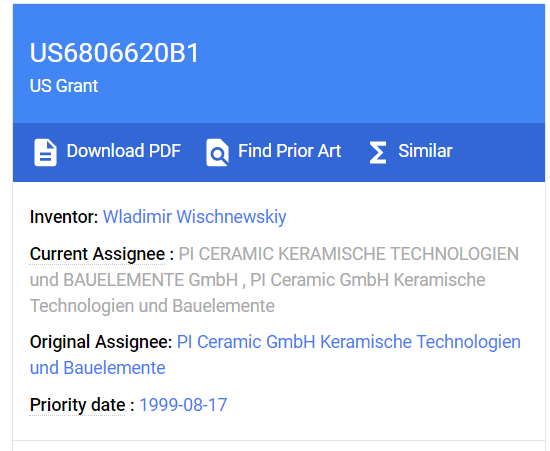
\includegraphics[width = 0.5\textwidth]{images/prilE} 
	\label{prilE}
\end{figure}

The invention relates to a piezoelectric drive, in particular for the generation of rotational and translational movements which can be carried out continuously or stepwise.\par

The inventive motor can be employed in automation systems, in robot technology, as a drive for microscope tables, for fine-positioning of various types of coordinate tables, in optical and laser systems, as well as in numerous other devices in which translational movements with high precision accuracy are required.\par

Piezoelectric motors or drives which are based on the utilisation of acoustic transducer travelling waves have been known for a longer period, with reference being made here for example to EP 0 475 752 and U.S. Pat. No. 5,596,241. Such motors, however, have the drawback that it is not possible to manufacture them as miniature drives, because the minimum length of the waveguide of these motors must be a multiple of 6? to 10?. In addition, the manufacture is complicated and expensive.\par

Such motors are relatively small and their manufacture is simple. A monolithic plate-shaped piezoelectric oscillator with a long and a short side and with a friction element which is arranged on one of its small surfaces is used as the drive element in such motors.\par

One of the large surfaces of the piezoelectric oscillator carries a first and a second electrode group. On the second one of the oscillator surfaces a continuous electrode is arranged. Each of the first and the second electrode group represents two equally sized diagonally arranged rectangular areas of the metallised piezoelectric ceramic surface. The source of the electric excitation of acoustic oscillations directs the voltage to the continuous electrode and to the first or second electrode group.\par


